\section{Introduction}
\label{intro}
With the rapid growing number of open datasets, data lake becomes a prevalent storage architecture across governments \cite{deng2024lakebench}, data scientists \cite{zhang2020finding}, businesses \cite{halevy2016goods} and enterprises\cite{khatiwada2022integrating}. Web tables constitute a substantial portion of data lakes due to their rich knowledge and semi-structured format \cite{deng2024lakebench}. In the Semantic Web community, table interpretation, tabular entity linking, semantic description induction, and dataset discovery have been extensively studied for exploiting tabular and dataset-level semantics~\cite{bhagavatula2015tabel,efthymiou2017matching,cutrona2020tough,vu2021graph,benjelloun2020google}. Among these tasks, table union search aims to retrieve tables that are unionable with a given query table, serving as a cornerstone for data integration and dataset enrichment \cite{nargesian2018table,zhang2020finding,leventidis2024large}. 

However, tables in data lakes are highly heterogeneous and large-scale, posing challenges to both effectiveness and efficiency. Early approaches design heuristic scoring functions to measure unionability but struggle to capture implicit semantics and structural heterogeneity \cite{nargesian2018table}. Recent representation learning methods leverage pre-trained language models to encode table semantics, with Starmie \cite{fan2022semantics} adopting contrastive learning and a filter–verification framework to compute unionability scores.
\begin{figure}[t]
    \centering
    
    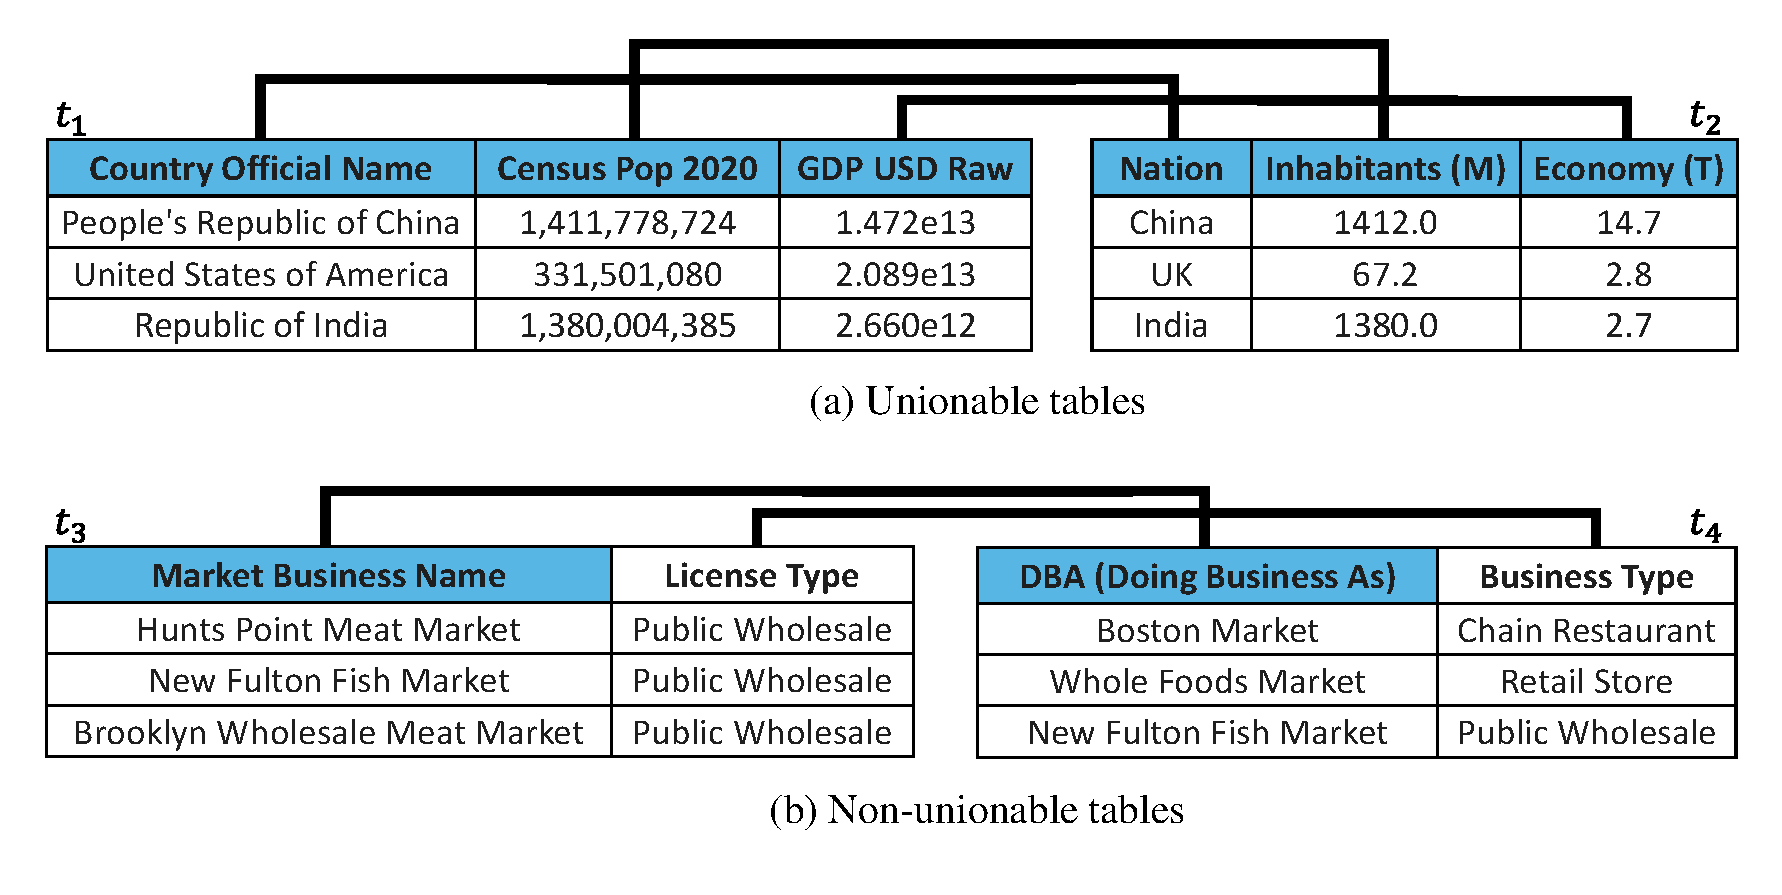
\includegraphics[width=\columnwidth]{figure/intro_example.pdf}
    
    \caption{An example of table union search. The black lines represent the matched columns.}
    
    \label{intro_example}
\end{figure}

Contrastive learning methods provide a self-supervised approach that resolves the lack of a large number of labels for training in table union search, thereby enhancing generalization \cite{fan2022semantics}. However, contrastive learning poses two challenges for table union search: (1) \textit{Implicit representation of semantic specificity.} Most approaches use deterministic point embeddings to encode tables or columns, modeling only semantic centers while ignoring semantic coverage. As illustrated in Figure \ref{intro_example}(b), columns {``Market Business Name''} in $t_3$ and {``DBA (Doing Business As)''} in $t_4$ may refer to the same entity type yet differ in specificity (wholesale markets vs. general markets). When represented as point vectors, such concepts may lie close in embedding space, leading to overestimated unionability. Without explicitly modeling semantic coverage, the boundary between general and specific concepts becomes blurred, resulting in unreliable retrieval decisions; (2) \textit{Self-referential bias in contrastive learning.} Standard contrastive frameworks assume that for an anchor table $t_i$, only its augmented view $t_i'$ is a positive sample, while all other tables are treated as negatives. This closed-world assumption introduces self-referential bias in heterogeneous data lakes \cite{boutaleb2025something}, where semantically compatible tables may coexist without explicit labels. Consequently, unionable tables (e.g., $t_1$ and $t_2$ in Figure \ref{intro_example}(a)) may be penalized as negatives, causing the model to overemphasize self-content and misclassify semantically related but lexically distinct tables.

To address the challenges identified earlier, this paper introduces the \underline{D}ual-\underline{G}ranularity \underline{G}aussian \underline{C}ontrastive Learning (DGGC) framework for table union search. DGGC models both tables and columns as Gaussian embeddings, where mean vectors capture semantic centers and variance vectors quantify semantic specificity. To ensure consistency between global table semantics and local column semantics, DGGC incorporates a table–column alignment objective within a unified Gaussian contrastive learning framework. 
Moreover, we design a filter–shuffle sample generator that constructs diverse inter-table positive pairs by filtering irrelevant tables and shuffling rows within unionable pairs. By extending positive supervision beyond self-augmentation, this strategy mitigates self-referential bias. Extensive experiments on three real-world corpora demonstrate that DGGC consistently improves union search effectiveness while maintaining efficiency.

The main contribution of this paper are summarized as follows:

\noindent $\bullet$\textit{Dual-Granularity Gaussian Contrastive Learning.} We introduce a Gaussian-based contrastive framework that explicitly models semantic specificity distributions at both table and column levels.

\noindent $\bullet$\textit{Filter-Shuffle Sample Generator.} We propose a positive sample generation strategy that constructs inter-table positives to alleviate the self-augmentation limitation in contrastive learning.

\noindent $\bullet$\textit{Experiment Results.} Experiments on three table corpora demonstrate consistent improvements over state-of-the-art methods, supported by ablation studies and case analyses. The reproducibility package is described in the Supplemental Material Statement and code are released in \small{https://anonymous.4open.science/r/DGGC-anonymous-artifact-7A99}. 


The remainder of the paper is organized as follows. Section~\ref{rel_work} reviews related work, Section~\ref{method} presents the proposed method, Section~\ref{exp} reports experimental results, and Section~\ref{cld} concludes the paper.

